\section{Introduction}
\label{sec:intro}
Large language models (LLMs) are increasingly used as natural-language (NL) interfaces for querying tabular data, making Table Question Answering (Table QA) a testbed for evaluating evidence retrieval, numerical operations, and analytical reasoning over structured information. However, most evaluations assume that structure is explicit, as in clean relational schemas, while many spreadsheets and reports use \emph{non-relational} tables whose structure is encoded in the presentation itself: hierarchical headers, merged cells, blank regions, unit conventions, noisy entries, or implicit dependencies between cells~\cite{1.10}.

This creates a blind spot in current Table QA evaluation. What is missing is a controlled instrument that keeps the underlying evidence and answer fixed while varying how evidence is presented, perturbed, and distributed across tables. A model may answer correctly over a clean relational table, but fail when the same latent information is rendered as a non-relational view. As shown in \autoref{fig:nonrelhurts}, and further detailed in \S\ref{app:generating_non_rel}, models consistently lose accuracy under non-relational renderings, with substantially larger drops in the multi-table setting. Manual construction is expensive because it requires designing realistic tables, questions, perturbations, units, missing values, and gold answers together; this limits scale, domain coverage, and diagnostic control.

%    Large language models (LLMs) are increasingly used as natural-language (NL) interfaces for querying tabular data. This makes Table Question Answering (Table QA) a testbed for evaluating whether models can retrieve evidence, perform numerical operations, and answer analytical questions grounded in structured information. However, much of the existing evaluation still assumes that the relevant structure is explicit: tables expose clean, relational schemas. In contrast, many spreadsheets, and reports use \emph{non-relational} tables, where the structure needed to answer a question is encoded in the presentation itself through hierarchical headers, merged cells, blank regions, unit conventions, noisy entries, and implicit dependencies between cells \cite{1.10}.

\begin{figure}[t]
    \centering
    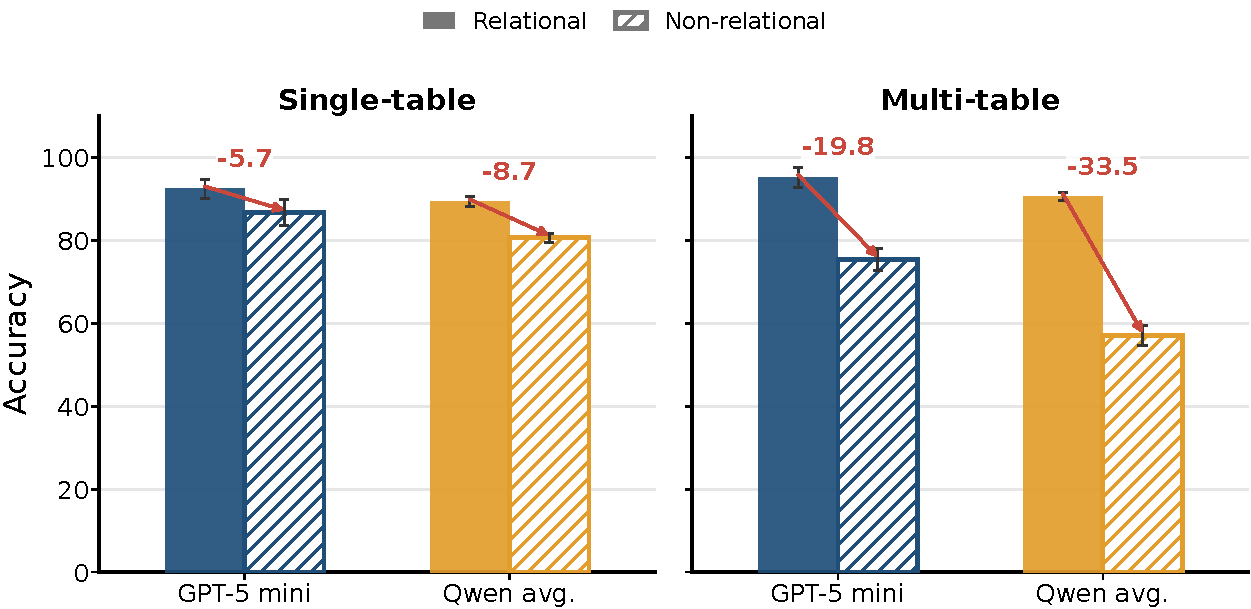
\includegraphics[width=0.48\textwidth]{img/rel_to_nonrel.pdf}
%    \caption{Absolute Table QA performance of \texttt{gpt-5-mini} and Qwen-family models on a sample of 200 questions built from tables extracted from Spider and Kaggle datasets. Each question was evaluated on both relational and non-relational variants of the same underlying data in both single- and multi-table settings.}
    \caption{Motivating comparison between relational and non-relational presentations: each question evaluated on the two variants %relational and non-relational variants 
    of the same underlying data in both single- and multi-table settings. Absolute Table QA performance of \texttt{gpt-5-mini} and Qwen-family on a sample of 200 questions %built 
    from %tables extracted from 
    Spider and Kaggle datasets.}
    % Red arrows indicate the corresponding performance degradation.
    \label{fig:nonrelhurts}
\end{figure}

\begin{figure*}[t]
    \centering
    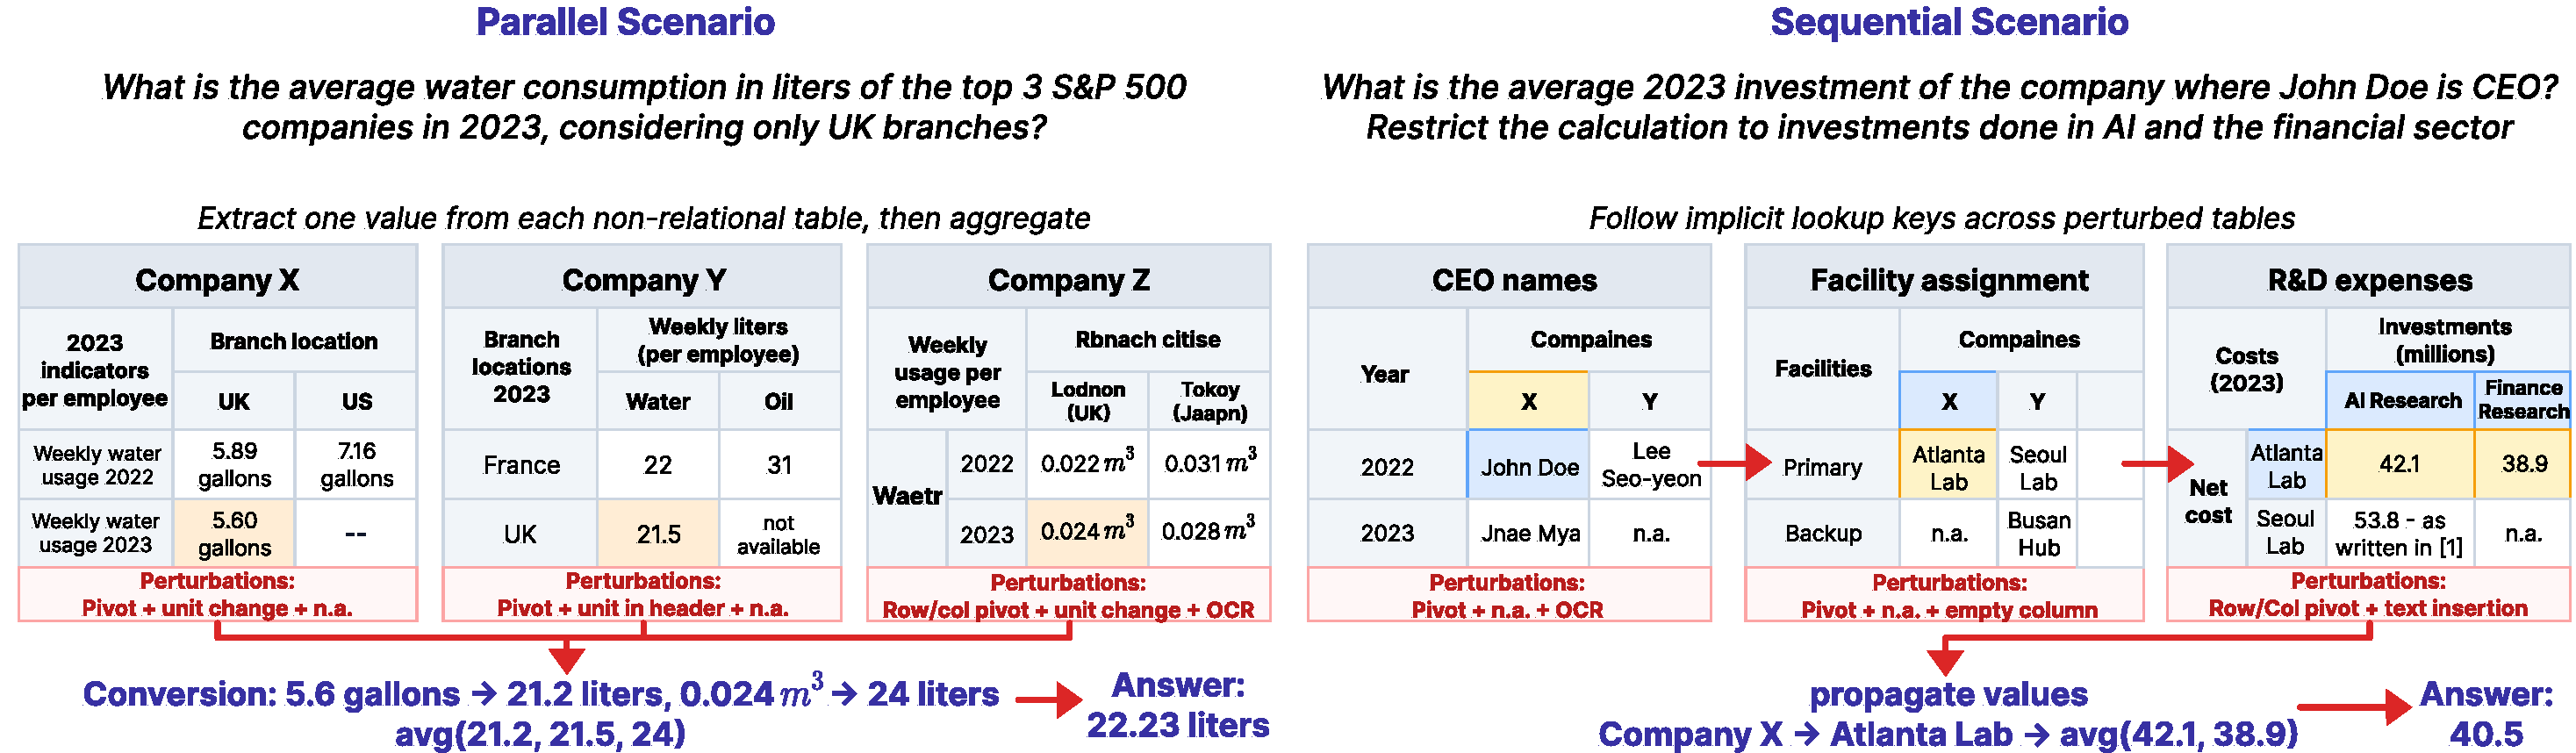
\includegraphics[width=0.99\textwidth]{img/q_types.pdf}
    % \caption{Examples of parallel and sequential scenarios generated by \name over multiple non-relational tables. Parallel questions require extracting and aggregating values across perturbed tables, while sequential questions require propagating lookup keys across tables before aggregating the final values.}
\caption{Multi-table parallel and sequential scenarios generated by \name over non-relational tables. Parallel questions extract and aggregate values across perturbed tables; sequential questions propagate lookup keys across tables before aggregating final values.}
    \label{fig:questiontypes}
\end{figure*}

% This creates a blind spot in current Table QA evaluation. \fg{What is missing is not only a harder collection of tables, but an evaluation instrument that can keep the underlying evidence and answer fixed while systematically varying how that evidence is presented, perturbed, and distributed across tables.} A model may answer a question correctly when the data is presented as a clean relational table, but fail when the same latent information is rendered as a non-relational table.%The problem becomes especially delicate in multi-table settings, where the model must not only interpret each table layout, but also determine how evidence should be combined across tables. 
% As shown in \autoref{fig:nonrelhurts}, non-relational presentation changes already degrade performance, and the degradation is substantially larger when the question requires reasoning over multiple tables.
% Lascerei solo caption \mpaga{As shown in \autoref{fig:nonrelhurts}, we evaluate 200 questions derived from tables extracted from Spider, BIRD, BEAVER, and Kaggle, transformed to support both non-relational formats and multi-table splits. Results show that GPT-5 mini and Qwen-family models degrade by about 6–9 points in single-table settings when moving from relational to non-relational tables. In the multi-table setting, this degradation becomes substantially larger, reaching about 20-35 points.}
% As shown in \autoref{fig:nonrelhurts}, and further detailed in \S\ref{app:generating_non_rel}, models consistently lose accuracy when relational tables are rendered as non-relational views, with substantially larger drops in the multi-table setting.
%Building such benchmarks requires annotated data in which questions, tables, and gold answers are known. %Such data are useful for testing and potentially also for training. 
% Building such benchmarks manually is expensive: one must design realistic tables, write questions, introduce layout and cell-level variation, handle units and missing values, and still guarantee that the final answer remains correct. \fg{This cost also makes it difficult to perform diagnostic evaluations: for example, to determine whether a model fails because of the layout, the number of tables, the unit convention, or their interaction.} This limits the scale, domain coverage, and diagnostic control of manually curated non-relational Table QA benchmarks.

% Building such benchmarks requires annotated data in which questions, tables, and gold answers are known. %Such data are useful for testing and potentially also for training. 
% However, manual construction is expensive: one must design realistic tables, write questions, introduce layout and cell-level variation, handle units and missing values, and still guarantee that the final answer remains correct. This cost limits the scale, domain coverage, and diagnostic control of manually curated non-relational Table QA benchmarks. 
% \mpaga{continuiamo ad ignorare l'esistenza di benchmark di TQA su tabelle non-relazionali...sec me occorre citare quelli esistenti (sia single che multi-table) e poi specificare che nonostante esistano, non è detto che esistano per tutti i domini o siano inerenti ad un dominio di interesse....una possibile soluzione potrebbe essere partire da una base relazionale, ed applicare metodi di automatic benchmark generation tramite trasformazioni controllate} \mlc{sono d'accordo sull'aggiungere una qualche frase di confronto con benchmark non-relazionali esistenti: ci sta focalizzarsi sul numero limitato di domini, ma allo stesso tempo mi focalizzerei anche sul numero di tabelle che nei benchmark esistenti è limitato (scaling collapse) e controllo sulle perturbazioni (nei dataset esistenti è difficile analizzare il comportamento di un modello su una perturbazione, in quanto esse difficilmente sono annotate). Non sono d'accordo sul partire dalla base relazionale, in quanto nei risultati discutiamo di come alcune perturbazioni non siano applicabili, quindi andremmo a contraddirci.}

\eat{
\mpaga{An alternative direction is to rely on existing non-relational Table QA benchmarks. While several datasets span different domains, such as finance, science, and environmental reporting (see \S\ref{sec:rw} for a comprehensive discussion), a suitable benchmark may not exist for a specific target domain. Moreover, even when available, these resources often differ from the intended use case: only a limited number are truly multi-table~\cite{1.26,1.16}, and the distribution of questions may not align with realistic user queries.}
% A natural alternative is automatic benchmark generation. \mpaga{Trovo un po' decontestualizzato questo aspetto della data contamination all'interno del discorso....mi sarei aspettato direttamente la discussione su metodi per la generazione di benchmark su tabelle relazionali} 
\mpaga{This has motivated automatic benchmark generation as a more scalable alternative, also helping mitigate data contamination issues when evaluating recent LLMs~\cite{datacontamination}.}
% Prior work has evaluated table reasoning through Table QA and Text-to-SQL benchmarks \cite{1.6,1.20,1.30}, which test whether models can generate executable SQL queries. Because these benchmarks are public and widely used, evaluating recent LLMs on them also raises contamination concerns \cite{datacontamination}. 
% This has motivated automatically generated benchmarks that 
Existing approaches extend semantic parsing datasets by generating templated multi-table SQL queries~\cite{PapicchioPC23}, others exploit database constraints to create automatically verifiable questions~\cite{5.5}; and further methods synthesize SQL programs over structured table--text collections \cite{5.8}. 
% These approaches improve scalability and verifiability \mpaga{faccio fatica a cogliere l'aspetto di verificabilità} \mlc{verifiability -> ogni gold label è ottenuta tramite esecuzione della query SQL, quindi è corretta (e verificabile) per costruzione}, but they inherit the structure of the underlying sources: schemas are explicit, join paths are known \mpaga{si intende che si conoscono PK e FK?} \mlc{effettivamente la frase è un po' imprecisa: l'idea è che l'estrazione delle foreign key constraints è più semplice su casi rel che non-rel a causa della struttura semplificata delle tabelle}, and the possible questions are bounded by the available relations \mpaga{cosa si intende?} \mlc{che con quegli approcci è impossibile fare domande che richiedono un numero potenzialmente illimitato di tabelle in input, in quanto il numero di tabelle è limitato dallo schema stesso del db (vedere bounded/unbounded in tabella 1)}. \mpaga{Sec me il paragrafo precedente va reso più chiaro: esistono metodi per automatic benchmark generation da tabelle relazionali, che sono limitati/vincolati alla struttura relazionale e aspetti derivati}
\mpaga{These techniques improve scalability and enable automatic answer verification. However, they remain inherently tied to the structure of relational sources: they assume explicit schemas, where schema matching and join discovery are considerably easier and unambiguous than in non-relational tables, and constrain the space of possible questions to those expressible within a fixed database schema, limiting support for more flexible or unbounded multi-table settings.}}

As manually curated tabular benchmarks also raise contamination concerns~\cite{datacontamination}, automatic benchmark generation is a natural alternative. Existing generators create templated multi-table SQL queries~\cite{PapicchioPC23}, use database constraints for verifiable questions~\cite{5.5}, or synthesize SQL programs over structured table--text collections~\cite{5.8}. However, they remain tied to relational sources, with explicit schemas, predefined join paths, and questions constrained by existing database relations. Non-relational Table QA benchmarks span domains such as finance, science, and environmental reporting (see \S\ref{sec:rw}), but are manually curated, fixed in domain and question distribution, and only rarely target genuinely multi-table reasoning~\cite{1.26,1.16}. They therefore offer limited control over table count, reasoning regime, perturbation type, and target domain.

% As manually-curated tabular benchmarks also raise contamination concerns~\cite{datacontamination}, a natural alternative is automatic benchmark generation. Existing generators create templated multi-table SQL queries~\cite{PapicchioPC23}, use database constraints for verifiable questions~\cite{5.5}, or synthesize SQL programs over structured table--text collections~\cite{5.8}. Yet they remain tied to relational sources, with explicit schemas, predefined join paths, and question spanning a limited amount of existing database relations. Non-relational Table QA benchmarks, on the other hand, span domains such as finance, science, and environmental reporting (see \S\ref{sec:rw}), but they are manually curated, fixed in domain and question distribution, and only rarely target genuinely multi-table reasoning~\cite{1.26,1.16}. They therefore provide limited control over the number of tables, reasoning regime, perturbation type, and target domain.

%, despite prior work \cite{1.16} showing that domain variation can substantially affect question answering performance.

% Existing non-relational Table QA benchmarks span domains such as finance, science, and environmental reporting (see \S\ref{sec:rw}), but they are manually curated, fixed in domain and question distribution, and only rarely target genuinely multi-table reasoning~\cite{1.26,1.16}. They therefore provide limited control over the number of tables, reasoning regime, perturbation type, and target domain.
% Automatic benchmark generation offers scalability and verifiability, and can reduce contamination risks for recent LLMs~\cite{datacontamination}. Existing generators create templated multi-table SQL queries~\cite{PapicchioPC23}, use database constraints for verifiable questions~\cite{5.5}, or synthesize SQL programs over structured table--text collections~\cite{5.8}. Yet they remain tied to relational sources, with explicit schemas, predefined join paths, and question spaces bounded by existing relations. They therefore do not provide the control needed for multi-table non-relational QA, where evidence is distributed across perturbed views and linked through layout, semantics, or unit normalization.

% \mpaga{Al fine di generare benchmark} For non-relational multi-table QA, \mpaga{partire da tabelle relazionali} this is insufficient for three reasons. First, existing relational tables often cannot be rendered into realistic non-relational layouts without invalid transformations \mpaga{cosa si intende per invalid transformations?} \mlc{l'idea è quella descritta in \autoref{fig:real_table_feasibility} e nel suo paragrafo ("Perturbed parallel and sequential questions are difficult to synthetize from real tables")} or substantial manual repair; in our experiments, many tables \mpaga{si può quantificare?} \mlc{vedere \autoref{fig:real_table_feasibility} per esempio di drop con pivot} from Spider, BIRD, and BEAVER \mpaga{mettiamo le ref?} do not support the required perturbations \mpaga{Sec me bisogna spiegare meglio: non hanno caratteristiche che le rendono candidate per essere trasformate in non-relazionali e quindi indicare un esempio}. Second, realistic multi-table questions do not follow a single join pattern \mpaga{tipico dei benchmark relazionali} \mpaga{Non sono sicuro che sia solo una questione di single/multi-way join...nel nostro caso subentra join su aggregazioni intermedie...sec me occorre stressare questa cosa perché se lo si presenta solo in termini di singl/multi-way già i benchmark relazionali lo supportano} \mlc{sono d'accordo, nel caso si cancella "single" o intendi altro? L'idea come hai detto e come è scritto sotto è quella di indicare, come vantaggio, lo scenario parallel (aggregazione)}. Some require \emph{parallel} reasoning, where the model aggregates \mpaga{matching} values from independent tables, often after resolving unit or numerical-format differences \mpaga{le differenze di unit e formato è molto buttato lì}. Others require \emph{sequential} reasoning, where the \mpaga{reasoning} model \mpaga{richiede di matchare risultati di aggregazioni intermedie} propagates intermediate entities or lookup keys across tables. %, and where links must be recovered semantically rather than through explicit foreign keys. 
% \autoref{fig:questiontypes} illustrates both regimes. Third, \mpaga{mentre le tabelle di benchmark relazionali fanno riferimento allo stesso database, applicare reasoning multi-tabella in scenario non-relazionale coinvolge spesso tabelle da diversi database ognuno col proprio formato/codifiche/etc.} tables can encode the same latent data in many surface forms: through pivots, nested headers, column merging, blank rows or columns, text insertions, typographical noise, missing values, and unit changes. A useful benchmark must vary these presentations independently while preserving the gold answer. 
% \mpaga{Arrivati a questo punto mi sembra chiaro che partire da tabelle relazionali non sia possibile per generare un benchmark non-relazionale, però se non ricordo male noi prendiamo anche in input delle tabelle relazionali....non ci stiamo contraddicendo?} \mlc{sì, ma solo per indicare che il drop in performance esiste anche con tabelle vere. Quelle che usiamo hanno passato una fase di filtering che ne ha droppate >95\%, quindi non è possibile partire da tabelle relazionali in quanto ci sarebbe un controllo pressochè nullo su domini delle tabelle (in quanto tante vengono droppate), question topology etc. \autoref{fig:real_table_feasibility}, \autoref{fig:rel_to_nonrel}}
\eat{
\mpaga{For non-relational multi-table QA, constructing benchmarks by starting from relational tables is insufficient for three main reasons. First, many relational tables cannot be meaningfully transformed into realistic non-relational layouts. For instance, among 2,096 tables extracted from the Spider, BIRD, and BEAVER databases, only 148 are sufficiently large ($\geq 3$ columns and $\geq 9$ rows) and contain at least one floating-point attribute to enable pivot-based transformations; when further restricting to dense pivotable tables (i.e., without introducing null entries), the selection drops to just 7 tables.}
\mpaga{Second, they differ in how cross-table links are established: relational settings rely on explicit schema-level keys enabling deterministic single-way or multi-way joins, whereas non-relational settings require semantic matching over heterogeneous and noisy representations, leading either to independent evidence aggregation or to propagation of intermediate entities via approximate rather than exact joins. We refer to these two paradigms as \emph{parallel} and \emph{sequential} settings, illustrated in \autoref{fig:questiontypes}.}
\mpaga{Third, unlike relational benchmarks where all tables share a unified schema and consistent encoding conventions, non-relational scenarios involve heterogeneous sources with diverse layouts and value representations. The same latent information may appear in multiple surface forms, including pivoted structures, nested or hierarchical headers, merged cells, blank rows or columns, textual noise, missing values, and unit inconsistencies.}
A useful benchmark must vary these presentations independently while preserving the gold answer.}

% Moreover, existing relational datasets do not easily allow non-relational tabular synthesis.
% %Starting from existing relational datasets does not solve this problem.
% As we show in \S\ref{app:generating_non_rel}, only a small fraction of tables from Spider, BIRD, and BEAVER can be converted into dense pivoted or hierarchical layouts without invalid cells. Furthermore, satisfying the constraints needed for multi-table reasoning is even harder. Moreover, the target non-relational multi-tabular reasoning differs from relational joining: in \emph{parallel} settings, models aggregate independent evidence across tables, whereas in \emph{sequential} settings, they propagate intermediate entities through implicit semantic links rather than explicit keys (\autoref{fig:questiontypes}). Finally, non-relational scenarios introduce heterogeneous layouts, surface forms, and unit conventions that must be varied independently while preserving the gold answer.

% Moreover, existing relational datasets do not easily lend themselves to non-relational tabular synthesis. As we show in \S\ref{app:generating_non_rel}, only a small fraction of tables from Spider, BIRD, and BEAVER can be converted into dense pivoted or hierarchical layouts without invalid cells, and satisfying the constraints needed for multi-table reasoning is even harder. Beyond this practical obstacle, in multi-table non-relational settings, the target reasoning can be fundamentally different from relational joining. In \emph{parallel} settings, the evidence is partitioned across separate tables that share neither join keys nor a common schema, and each table exposes a single relevant value through its own layout and surface form. The model must therefore locate the corresponding scalar in each table independently and aggregate these values to obtain the answer (\autoref{fig:questiontypes}). In \emph{sequential} settings, the tables are linked, but only through implicit semantic correspondences rather than explicit keys, forcing the model to propagate intermediate entities across tables on its own. Finally, non-relational scenarios introduce heterogeneous layouts, surface forms, and unit conventions that must be varied independently while preserving the gold answer.

Moreover, existing relational datasets do not easily support non-relational synthesis. As we show in \S\ref{app:generating_non_rel}, only a small fraction of Spider~\cite{1.6}, BIRD~\cite{1.20}, and BEAVER~\cite{1.30} tables can be converted into dense pivoted or hierarchical layouts without invalid cells, and multi-table constraints are even harder to satisfy. Thus, relational datasets do not provide a flexible substrate for controlled non-relational benchmark generation. Beyond this practical obstacle, multi-table non-relational QA differs from relational joining: in \emph{parallel} settings, models aggregate independent evidence across tables that share neither join keys nor a common schema; in \emph{sequential} settings, they propagate intermediate entities through implicit semantic links rather than explicit keys (\autoref{fig:questiontypes}). A useful benchmark must also vary layouts, surface forms, and unit conventions independently while preserving the gold answer.

% Moreover, existing relational datasets do not easily lend themselves to non-relational tabular synthesis. As we show in \S\ref{app:generating_non_rel}, only a small fraction of tables from Spider, BIRD, and BEAVER can be converted into dense pivoted or hierarchical layouts without invalid cells, and satisfying the constraints needed for multi-table reasoning is even harder. \fg{Thus, relational datasets are useful for demonstrating that non-relational presentation hurts model performance, but they do not provide a sufficiently flexible substrate for controlled benchmark generation.} Beyond this practical obstacle, in multi-table non-relational settings, the target reasoning can differ from relational joining: in \emph{parallel} settings, models aggregate independent evidence partitioned across separate tables that share neither join keys nor a common schema, whereas in \emph{sequential} settings, they propagate intermediate entities through implicit semantic links rather than explicit keys (\autoref{fig:questiontypes}). Finally, non-relational scenarios introduce heterogeneous layouts, surface forms, and unit conventions that must be varied independently while preserving the gold answer.

To make such controlled evaluation possible, we introduce \name, a flexible from-scratch framework for generating automatically verifiable QA benchmarks over multiple non-relational tables.
\name requires only a target domain and lightweight generation controls from the user, such as attribute cardinalities and table count. \name then uses an LLM to generate a domain-specific schema, instantiates a \emph{latent relational source}, derives executable SQL supervision and scalar answers, and verbalizes the SQL programs into NL questions.

Starting from the latent source, \name generates the benchmark inputs: perturbed \emph{non-relational views}, i.e., table representations with controlled layout, noise, and numerical variation. These views combine perturbations previously shown to challenge relational QA models~\cite{2.4,2.5,2.6,2.8}, such as schema edits, distractors, and noisy or missing values, with transformations tailored to non-relational tables, including pivots, hierarchical headers, merged cells, layout restructuring, and unit conversions. In multi-table scenarios, \name also controls how evidence is distributed across views, supporting \emph{parallel} aggregation and \emph{sequential} propagation. %through implicit semantic links.
The core idea is to separate supervision from presentation: the latent relational source is used to compute and verify answers, while the perturbed non-relational views form the evaluation data shown to the model. %This lets \name vary reasoning topology, table count, perturbations, and answer distributions without changing the gold answers.
This lets \name vary reasoning topology, perturbations, and answer distributions while scaling the table count to arbitrarily high values, all without changing the gold answers.

% \mpaga{Starting from this latent source, \name automatically generates non-relational table representations and controlled multi-table settings by combining perturbations previously shown to challenge relational QA models~\cite{2.4,2.5,2.6,2.8}, such as schema edits, distractor attributes, and noisy or missing values, with additional structural and numerical transformations tailored to non-relational scenarios, including pivots, hierarchical headers, merged cells, layout restructuring, and unit conversions. In multi-table scenarios, \name further controls how evidence is distributed across tables, supporting both parallel settings, where evidence is aggregated independently, and sequential settings, where intermediate entities must be propagated across approximate semantic matches rather than exact relational joins.}

% \mpaga{The core design principle of \name is the separation between supervision and presentation. The latent relational source is used only as an internal executable layer for answer generation and verification, while models are evaluated exclusively on perturbed non-relational views derived from it. This separation enables independent control over reasoning topology, number of tables, perturbation strategies, and answer distributions, while preserving semantic consistency and gold answers across different renderings.}



% The key design choice is to separate supervision from presentation. The latent relational source is used only to compute and verify answers. Models are evaluated on perturbed \emph{non-relational views}: table renderings generated by \name from the same latent source and shown as input to the model. This separation allows \name to control the reasoning topology \mpaga{(i.e., parallel or sequential)}, number of tables, perturbation type \mpaga{esempio?}, unit setting, and answer distribution independently. It also allows structural, cell-level, and numerical perturbations to be applied without changing the underlying answer.

% We evaluate open and closed models on financial and environmental instances generated by \name. The results show that current LLMs remain brittle in this setting. Accuracy decreases sharply as the number of tables increases, especially when models must aggregate many evidence values or propagate implicit lookup keys across tables. \mpaga{Riporterei il numero massimo di tabelle che abbiamo generato per ogni domanda} Unit heterogeneity introduces additional domain-dependent failures, suggesting that robust Table QA evaluation should account for both reasoning topology and numerical conventions. Finally, although \name is primarily designed for controlled evaluation, we also show that generated instances can provide useful supervision: fine-tuning on \name data improves performance on GRI-QA \cite{1.16} compared to the non-finetuned Qwen baseline.

\begin{table*}[t]
\centering
\fontsize{8.8pt}{10pt}\selectfont
\setlength{\tabcolsep}{1.10pt}
\renewcommand{\arraystretch}{1.15}
\begin{tabular}{llccc cccc}
\toprule
\textbf{Class} &
\textbf{Approach} &
\multicolumn{3}{c}{\textbf{Generated artifacts}} &
\multicolumn{4}{c}{\textbf{Reasoning / evaluation control}} \\
\cmidrule(lr){3-5}
\cmidrule(lr){6-9}
& & Tbl. & NLQ & Ans. & Pert. & Rel. & Non-rel. & \# tables \\
\midrule
\multirow{4}{*}{Perturbation}
& Dr.Spider~\cite{2.6}   & \xmark & \xmark & \xmark & Sch/Txt/Cell & \checkmark & \xmark & Bounded \\
& EvoSchema~\cite{2.8}   & \xmark & \xmark & \xmark & Sch          & \checkmark & \xmark & Bounded \\
& ADVETA~\cite{2.5}      & \xmark & \xmark & \xmark & Sch          & \checkmark & \xmark & Bounded \\
& FREB-TQA~\cite{2.9}    & \xmark & \xmark & \xmark & Cell/Lay     & \xmark     & \checkmark & 1 \\
\midrule
\multirow{3}{*}{\makecell[l]{Tabular\\synthesis}}
& REaLTabFormer~\cite{5.9} & \checkmark & \xmark & \xmark & \xmark & \checkmark & \xmark & N/A \\
& GOGGLE~\cite{5.10}       & \checkmark & \xmark & \xmark & \xmark & \checkmark & \xmark & N/A \\
& TabGen-ICL~\cite{5.1}    & \checkmark & \xmark & \xmark & \xmark & \checkmark & \xmark & N/A \\
\midrule
\multirow{8}{*}{\makecell[l]{QA / SQL\\synthesis}}
& \citet{9.1}           & \xmark     & \xmark     & \checkmark & \xmark & \checkmark & \xmark & 1 \\
& \citet{9.2}           & \xmark     & \checkmark & \checkmark & \xmark & \checkmark & \xmark & 1 \\
& \citet{9.5}           & \xmark     & \xmark     & \checkmark & \xmark & \checkmark & \xmark & Bounded \\
& ER-Bench~\cite{5.5}   & \xmark     & \checkmark & \checkmark & \xmark & \checkmark & \xmark & Bounded \\
& SPARTA~\cite{5.8}     & \xmark     & \checkmark & \checkmark & \xmark & \checkmark & \xmark & Bounded \\
& DSQG-Syn~\cite{9.8}   & \xmark     & \checkmark & \checkmark & \xmark & \checkmark & \xmark & Bounded \\
& SQLForge~\cite{9.7}   & \checkmark & \checkmark & \checkmark & \xmark & \checkmark & \xmark & Bounded \\
& SYNQL~\cite{9.6}      & \xmark     & \checkmark & \checkmark & \xmark & \checkmark & \xmark & Bounded \\
\midrule
\textbf{Ours}
& \textbf{\name}
& \checkmark
& \checkmark
& \checkmark
& \textbf{Sch/Cell/Lay/Num}
& \checkmark
& \checkmark
& \textbf{Unbounded} \\
\bottomrule
\end{tabular}
\caption{
Comparison with benchmark and data-generation approaches.
Tbl., NLQ, and Ans. denote generated tables, natural-language questions, and automatically verifiable answers.
Perturbations are abbreviated as schema/name (Sch), text/query (Txt), cell/content (Cell), layout/structure (Lay), and numerical/unit (Num).
The number of tables is either fixed to one, bounded by an existing source, or generator-controlled. \name is the only approach to generate tabular benchmarks from scratch and apply perturbations without any constraint on the table number.
}
% \caption{
% Comparison with related benchmark and data-generation approaches.
% Under \textbf{Generated artifacts}, Tbl., NLQ, and Ans. indicate whether a method generates tables, natural-language questions, and automatically verifiable gold answers.
% Under \textbf{Reasoning / evaluation control}, Pert. summarizes the supported perturbation types: Sch = schema/name perturbations; Txt = natural-language or SQL/query perturbations; Cell = cell/content perturbations; Lay = layout or structural perturbations; Num = numerical or unit perturbations.
% Rel. and Non-rel. indicate whether the evaluated tables expose a clean relational-style schema or non-relational presentations.
% \#~tables indicates whether the number of tables per instance is fixed to one (1), bounded by an existing database (Bounded), or unbounded. \name is the only approach to generate tabular benchmarks from scratch and apply perturbations without any constraint on the table number. \mpaga{Mi domando, dal momento che sono pochi, se abbia senso introdurre nella tabella anche benchmark TQA su molteplici tabelle non-relazionali}
% }
\label{tab:related_work_comparison}
\end{table*}

We evaluate \name on financial and environmental scenarios with up to 20 parallel tables and 5 sequentially connected tables per question, using \texttt{gpt-5-mini} and Qwen-family models. Accuracy drops by 25--40 points as the number of tables increases; in the hardest settings, performance remains slightly above 60\% for parallel questions and often below 50\% for sequential ones. Unit heterogeneity compounds these drops, with domain-dependent effects of up to 50 points. 
%These results show that \name generates diverse, controlled benchmarks that challenge current LLMs by jointly varying reasoning topology, structural complexity, and numerical conventions. 
Although \name is primarily designed for controlled evaluation, we also find that generated instances can provide useful supervision: fine-tuning on \name-generated data improves performance on GRI-QA~\cite{1.16} compared to the non-finetuned Qwen baseline, especially when the generated data match the target domain.



% \mpaga{To evaluate \name, we generate multi-table TQA benchmarks with the proposed framework and analyze the performance of both open- and closed-source LLMs on complex reasoning scenarios involving up to 20 parallel tables and 5 sequentially connected tables per question across two domains: finance and environmental reporting.}

% \mpaga{Results show that \name can generate highly challenging scenarios for current LLMs. GPT-5 mini and Qwen-family models up to 122B parameters exhibit substantial performance degradation as the number of tables increases, with average drops in the range of 25–40 points and best-case accuracies only slightly above 60\% in parallel settings. Performance further deteriorates in sequential configurations, where accuracies fall below 50\%, highlighting the difficulty of propagating intermediate entities through approximate semantic matches across tables. We also observe that \name can inject domain-specific unit heterogeneity that further amplifies these effects. In the environmental domain, where unit transformations are more frequent, models experience additional degradations of around 40 accuracy points, resulting in absolute performance below 40\% in some cases. Overall, these findings show that \name can generate diverse and controlled benchmarks, effectively challenging current LLMs by jointly manipulating reasoning topology, structural variability, and numerical conventions within Table QA scenarios.}

% \mpaga{Finally, although \name is primarily designed for controlled evaluation, we demonstrate that it can also provide effective training supervision. Fine-tuning Qwen-14B on financial data generated by \name achieves performance comparable to training on real-world financial datasets such as TAT-QA, improving accuracy by approximately +10 points over a non-finetuned baseline. Similarly, in the environmental domain, training on \name-generated environmental data yields strong gains on GRI-QA, with improvements of about +17 points over the base model, compared to +25 points when using real-world supervision.}

In summary, our contributions are:
(i) we introduce \name, a from-scratch generator for automatically verifiable numerical QA over multiple non-relational tables;
(ii) we define two controllable multi-table reasoning regimes, parallel and sequential, together with answer-preserving structural, cell-level, and unit-based perturbations;
(iii) we use \name to evaluate recent LLMs in financial and environmental domains, showing that non-relational presentation, unit heterogeneity, and table count substantially degrade performance; 
(iv) we publicly release code and generated datasets\footnote{\href{https://anonymous.4open.science/r/Gradino-DBF6/}{Anonymous Github link}}.
%As an additional use case, we show that generated instances can also improve downstream Table QA training.